\documentclass[tikz]{standalone}
\usepackage{amsmath}
\definecolor{bg}{HTML}{171D2B}
\definecolor{aksen}{HTML}{F7B538}
\begin{document}
\pagecolor{bg}
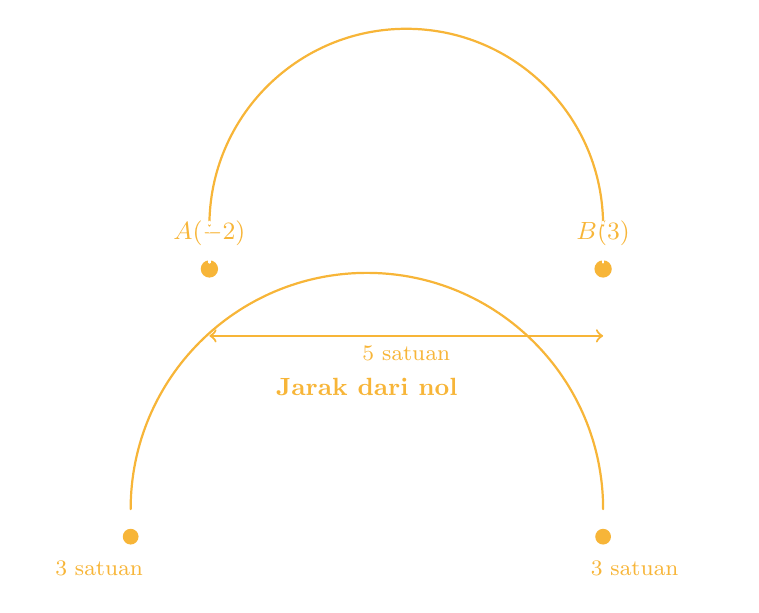
\begin{tikzpicture}[line cap=round, line join=round]
  \begin{scope}
    % garis bilangan utama
    \draw[white, very thick] (-4.2,0) -- (4.6,0);
    \foreach \x in {-4,...,4}
      \draw[white, thick] (\x,0.12) -- (\x,-0.12) node[below, text=white, font=\footnotesize] {$\x$};
    % titik A(-2) dan B(3)
    \fill[aksen] (-2,0) circle (0.11) node[above=5pt, text=aksen, font=\small] {$A(-2)$};
    \fill[aksen] (3,0) circle (0.11) node[above=5pt, text=aksen, font=\small] {$B(3)$};
    % busur jarak
    \draw[aksen, thick] (-2,0.55) arc[start angle=180, end angle=0, radius=2.5];
    \node[text=white, font=\small] at (0.5,1.15) {$|-2-3| = |-5| = 5$};
    \draw[white, dotted, thick] (-2,0.08) -- (-2,0.62);
    \draw[white, dotted, thick] (3,0.08) -- (3,0.62);
    % panah hitung langkah
    \draw[aksen, <->, thick] (-2,-0.85) -- (3,-0.85)
      node[midway, below, text=aksen, font=\footnotesize] {5 satuan};
  \end{scope}
  % panel bawah: |x| sebagai jarak dari 0
  \begin{scope}[yshift=-3.4cm]
    \node[text=aksen, font=\bfseries\small] at (0,1.9) {Jarak dari nol};
    \draw[white, very thick] (-4.0,0) -- (4.0,0);
    \foreach \x in {-4,...,4}
      \draw[white, thick] (\x,0.10) -- (\x,-0.10);
    \node[text=white, font=\footnotesize] at (0,-0.35) {$0$};
    \fill[aksen] (-3,0) circle (0.10);
    \fill[aksen] (3,0) circle (0.10);
    \draw[aksen, thick] (-3,0.35) arc[start angle=180, end angle=0, radius=3];
    \node[text=white, font=\small] at (0,1.15) {$|-3| = |3| = 3$};
    \node[text=aksen, font=\footnotesize] at (-3.4,-0.4) {3 satuan};
    \node[text=aksen, font=\footnotesize] at (3.4,-0.4) {3 satuan};
  \end{scope}
\end{tikzpicture}
\end{document}
